%!TEX root = ../master.tex
\chapter{Testing and Evaluation}\label{ch:testeval}
In order to evaluate the product and see to what extent it can be considered successful, a usability test will be conducted.

\section{Purpose of test}
The purpose of this test is to test usability and functionality of the product. The ISO 9241 \citep{ISO} standard defines usability as effectiveness, efficiency, and satisfaction of the user. Put more precisely, this means:
\begin{itemize}
\item Efectiveness: To what extent are the goals of the product achieved?
\item Efficiency: What resources (including time) are expended to achieve the goals?
\item Satisfaction: To what extent does the user find the system acceptable?
\end{itemize}
With these in mind, the test aims to clarify whether the product lives up to its test objectives.

\section{Test objectives}
\todo{Andreas snakkede om at splitte objektiverne op i tech/usability, men spørgsmålet er om usability er det rigtige at bruge her eller om vi skal holde os til satisfaction}The problem statement is defined in Section~\ref{sec:ProblemStatement}. Based on this problem statement, it is important not only to test how well the program functions on a technical level, but also if the test participants still feel like they are playing the original board game, which will be tested on a level of satisfaction/acceptance.
The success criteria (Section~\ref{sec:SuccessCriteria}) and the system requirements (Section~\ref{sec:ReqSpec}) each add to the specifications on the technical and satisfaction  objectives of the test.

The technical oriented test objectives are:\todo{Change these to the new technical objectives}
\begin{enumerate}
\item Does the player selection task live up to the requirement specification that it should be successful 90\% of the time?
\item Does the terraforming task live up to the requirement specification that it should be successful 90\% of the time?
\item What is the average delay time from the moment a gesture is done, to the moment the result can be seen on the interface?
\end{enumerate}
The satisfaction oriented test objectives are:
\begin{enumerate}
\item Do the players still feel like they are playing Terra Mystica, when they are playing the augmented version?
\item Do the players feel like taking turns using the player selection gestures is an easy task, or a hindrance?
\item Do the players feel like the task of terraforming is easier to carry out than on the original board game?
\item Do the players feel that the augmented game board can replace the original game board?
\item How do the gestures for player selection and terraforming affect the pace of the game?
\end{enumerate}

These objectives set the goals for the test, and help determine whether or not the test is successful. 

\section{Test methods}
To evaluate the product, two types tests are conducted. The first one is a technical tests using only group members, in order to test the technical aspects of the program, as this does not require participants from outside the group. The second type of test is the usability test, of which several will be conducted. These tests will focus on the satisfaction aspect of usability.

\subsection{Technical test}
\todo{technical test method goes here}

\subsection{Usability test set-up}
\begin{figure}
	\centering
	\begin{subfigure}[b]{0.4\textwidth}
	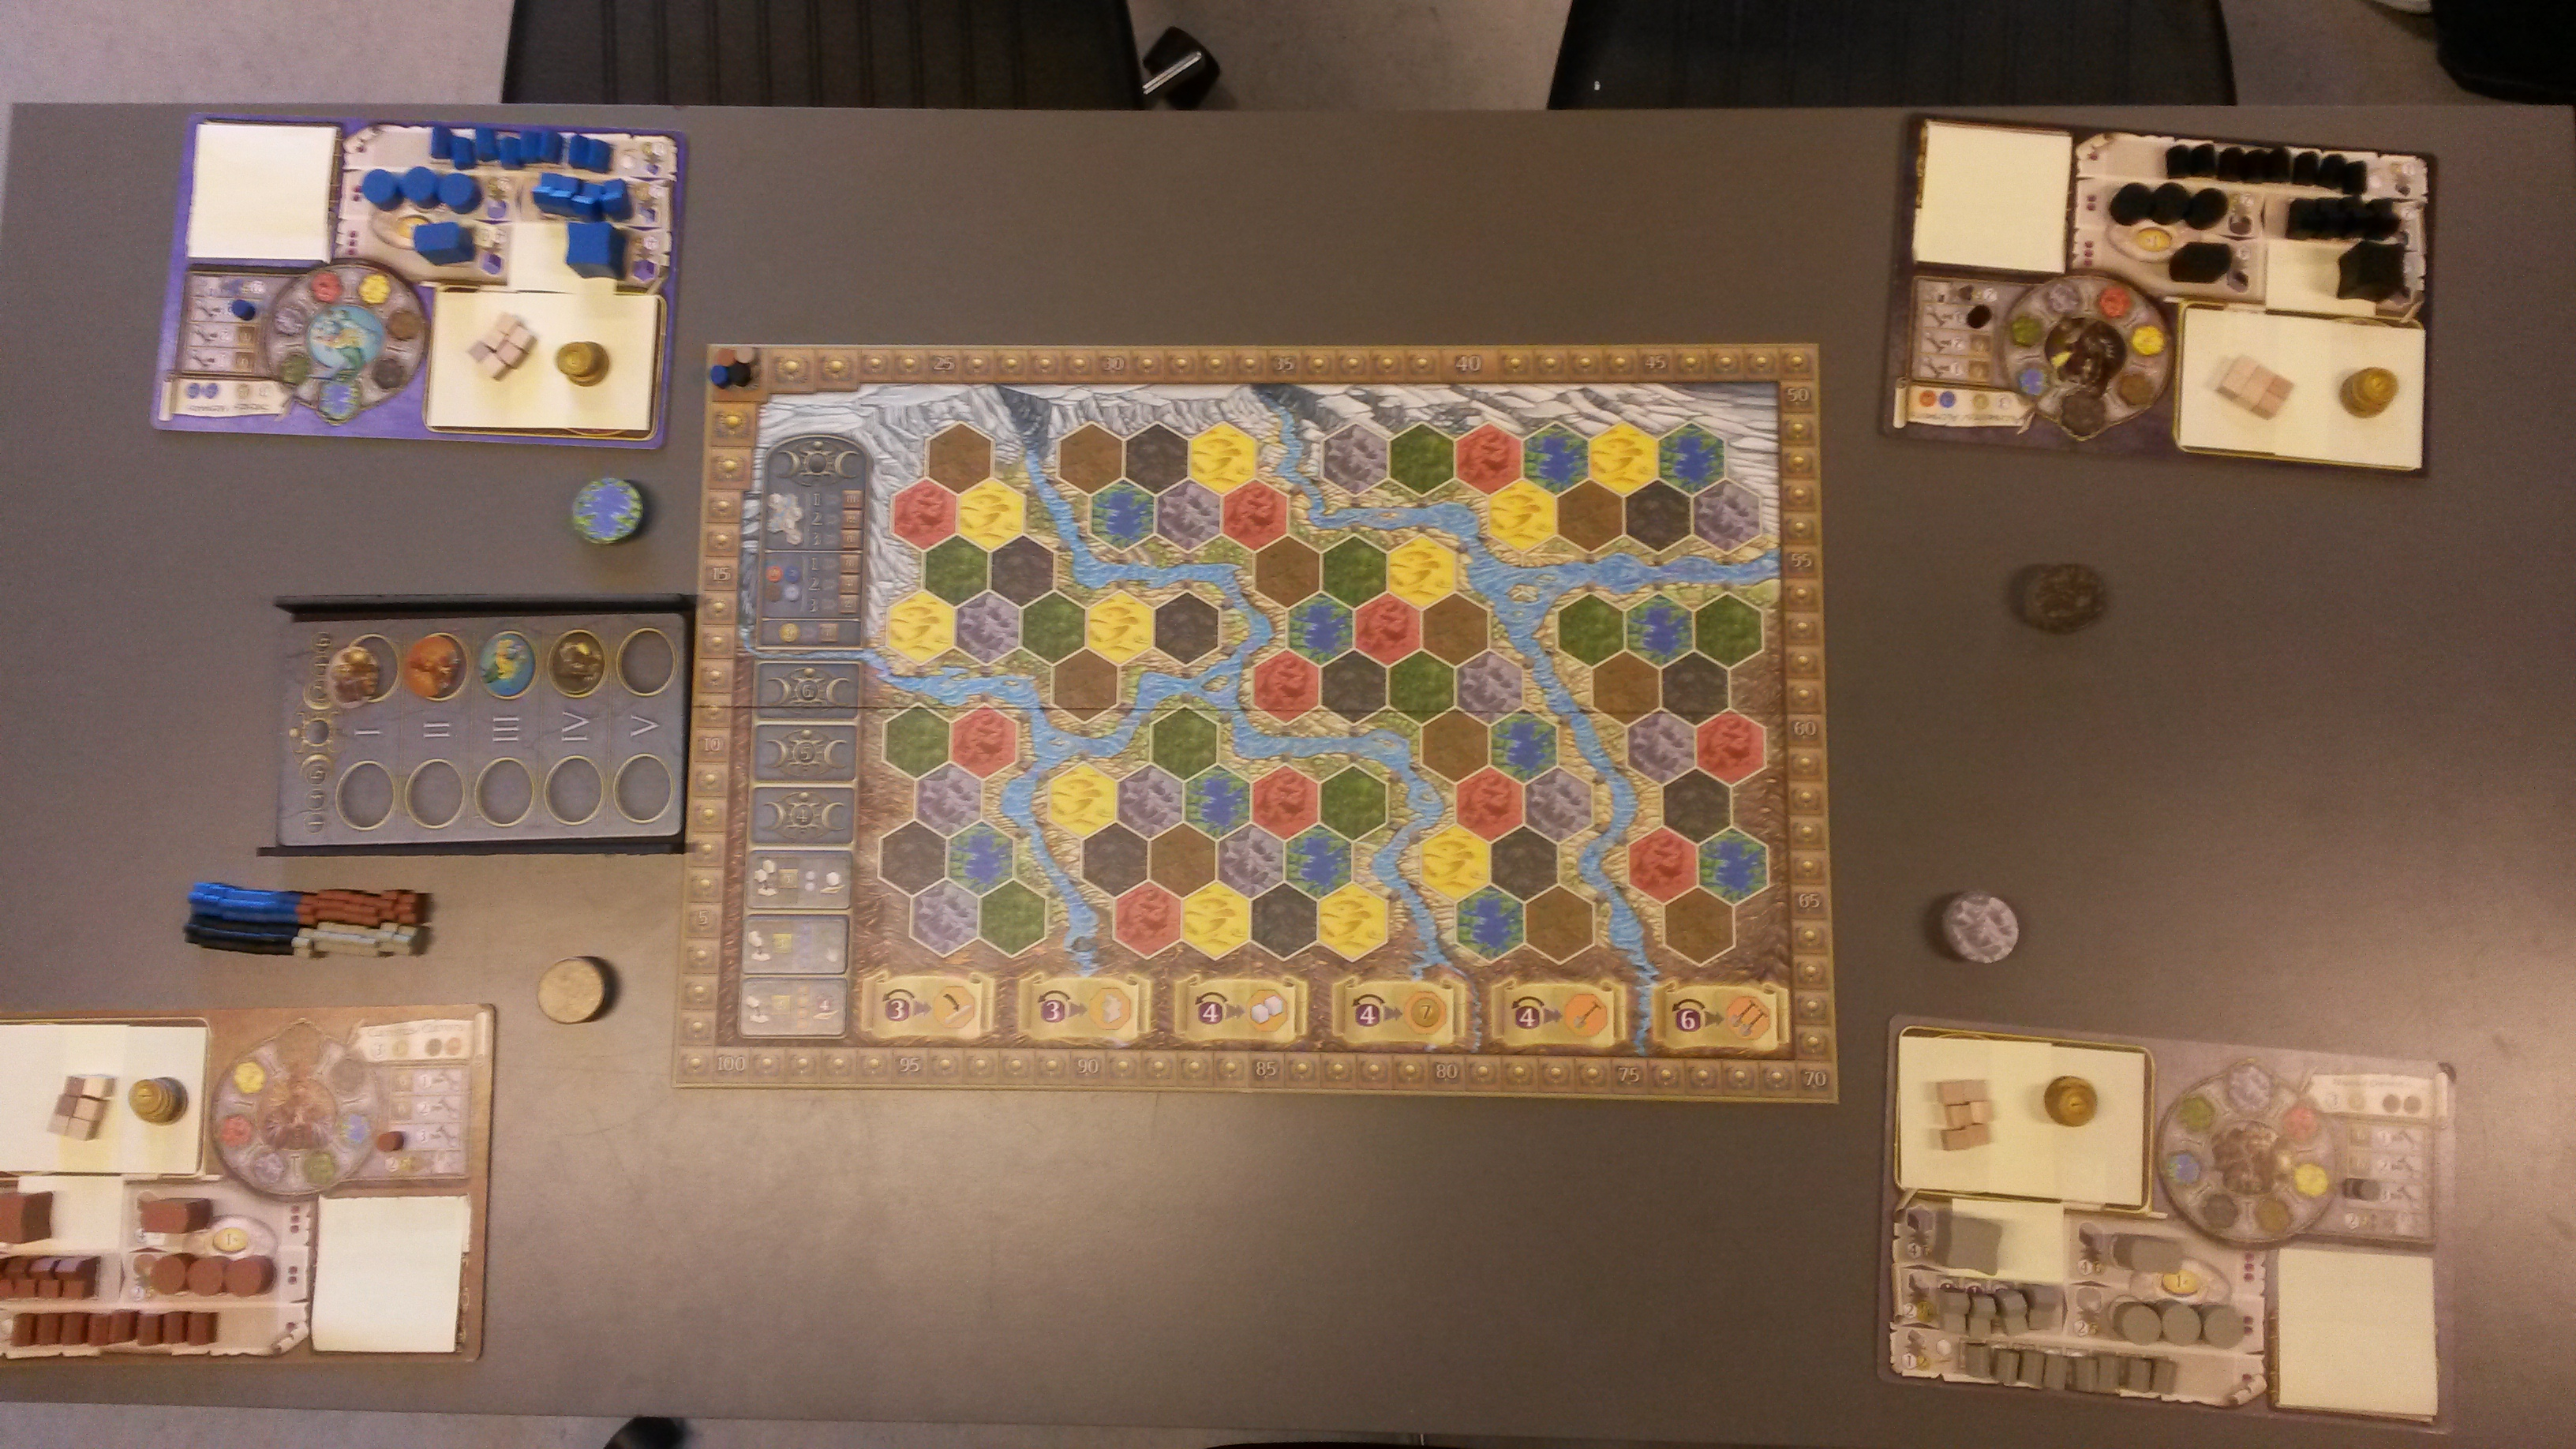
\includegraphics[width=\textwidth]{setup_analogue}
		\caption{\label{Fig:SetupAna}}
	\end{subfigure}
	\begin{subfigure}[b]{0.4\textwidth}
	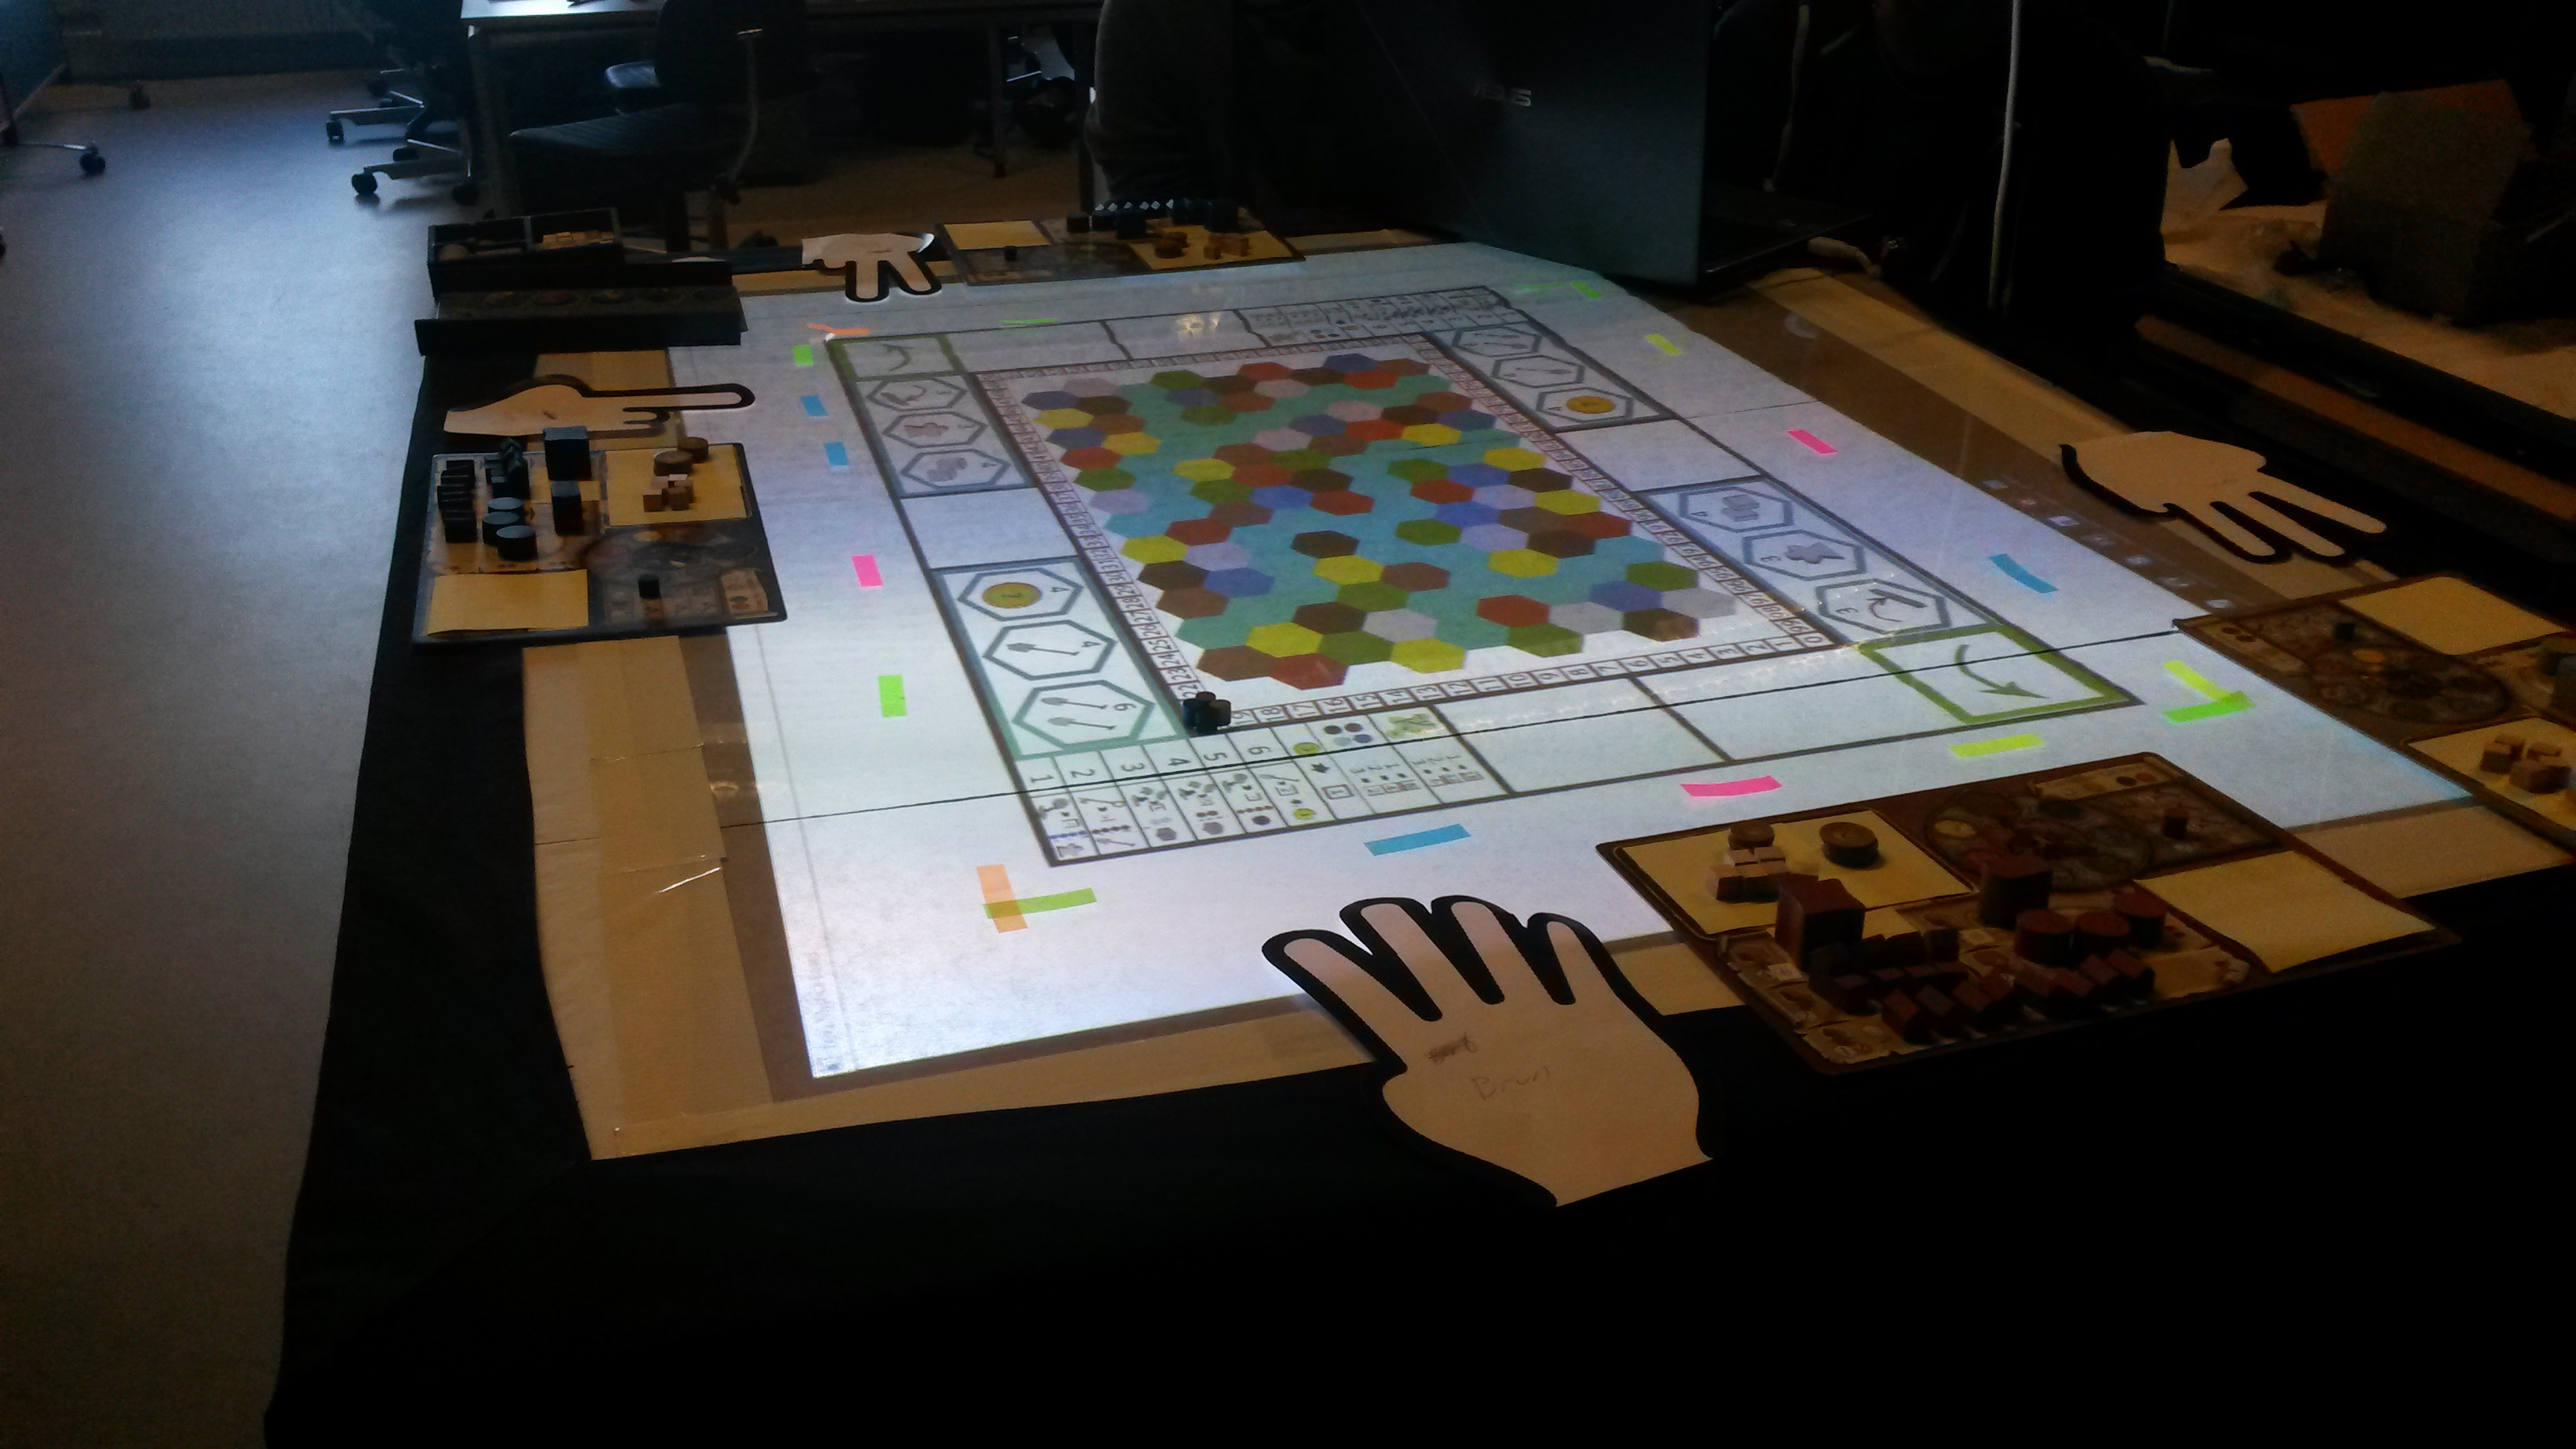
\includegraphics[width=\textwidth]{setup_digital}
		\caption{\label{Fig:SetupDigi}}
	\end{subfigure}
	\caption{Setup for the usability test, showing participants both the analogue game \textbf{(a)}, and the digital one \textbf{(b)}.\label{Fig:Setup}}
\end{figure}\todo{I don't know if we want these setup pictures or ones with participants on them. If we want the latter we can grab them from the video.}
The test takes place in the open study area, since the set-up requires a lot of room and the hardware will take up extra time to disassemble and reassemble, and moving it may dama the diffusor. Two tables are used for this test; one is the augmented board built for this project, and one is a table with the analogue game for comparison. The two setups can be seen in Figure \ref{Fig:Setup}. As the test includes people who are not experienced with Terra Mystica, several aspects of the game have been removed for simplicity's sake. These are covered up on each player's information board. Four test participants are placed around the table for each test, one by each information board, as well as four testers: One to operate a camera to record the test, one to take notes, one to explain the rules to the participants, and one to guide the participants and conduct the interview.
%The test will take place in a controlled setting, where nobody else besides the test participants and testers will be present around a board while a game is taking place. The participants will be playing, and the testers will only act as observers who document the proceedings, and helpers/guides - in case the participants have any technical problems that prevent them from proceeding from the test.
%The documentation of the test will be done by a tester filming the participants playing the game and a note-taker that also acts as the spokesperson for the testers.

\subsection{Participants for usability tests} \todo{maybe relocate this subsection further up}
The chosen test participants are 16 young adult students from the AAU and they are our typical users. They are within the target group, which is defined in Section~\ref{sec:TargetGroup}, meaning that they are experienced with board games. We do not base our test on all participants being familiar with Terra Mystica, and therefore based the test design on participants just being familiar with board games in general. 

\subsection{Procedure for usability test}\todo{there will be changes here later on the week}
The test, when set up, will follow this procedure:

\begin{enumerate}
\item To begin with, the test guide will introduce the participants to the game and the project product, and then explain the whole test procedure. The guide will have a script to read from, which can be found in Appendix \ref{ch:TestScript}, to make sure all participants are fully informed.
\item Once all participants understand the procedure, they will play a game of Terra Mystica either using the augmented or original board for 3 rounds. After those 3 rounds are over, the participants will play a game with the board they have not tried yet. \todo{question is if we should add questions in between the games, since not only their comparison, but also initial impression might have significance} During the test introduction, they are encouraged to have dialogues with each other regarding their actions and thoughts as they play. This is inspired by the think aloud method addressed by Larsen \citep{TestingLecture}. The whole test is filmed by the cameraman. It is especially important to get footage of the participants' hands as they attempt to do gestures and as the related actions in the original version. It is likely that all of the typical tasks will be performed during this playthrough, but if not, the test guide will ask the test participants to attempt the ones they forewent.
\item Once the practical part of the test is over, the test guide will conduct a semi-structured group interview, which the participants have been informed about during the introduction. The participants will be asked about how they experienced the augmented game, both in its own right, and in comparison to the original game.
\end{enumerate}

Once the test is done, the footage and notes from the test will be analysed and compared to the test objectives.

\section{Results}
\subsection{Technical}
\subsection{Satisfaction}
\subsection{Analysis}
text\todo{analysis and conclusion}